\documentclass[10pt,conference]{IEEEtran}

\ifCLASSINFOpdf
	\usepackage[pdftex]{graphicx}
	%\graphicspath{{./figs/}}
	\DeclareGraphicsExtensions{.pdf,.jpeg,.png,.jpg}
\else
	\usepackage[dvips]{graphicx}
	%\graphicspath{{./figs/}}
	\DeclareGraphicsExtensions{.eps}
\fi
\usepackage{float}
\usepackage{bm}
% \usepackage{amsmath}
\usepackage{amssymb}
\usepackage{graphicx}
\graphicspath{ {images/} }
\usepackage[cmex10]{amsmath}
\usepackage[tight,footnotesize]{subfigure}
\usepackage{xcolor}
\usepackage[lined,ruled]{algorithm2e}
\usepackage[latin1]{inputenc}
\usepackage{tikz}
\usetikzlibrary{shapes}
\usetikzlibrary{arrows}

\usepackage[]{algorithm2e}

\newtheorem{property}{Property}
\newtheorem{proposition}{Proposition}
\newtheorem{theorem}{Theorem}
\newtheorem{conjecture}{Conjecture}
\newtheorem{question}{Question}
\newtheorem{definition}{Definition}
\newtheorem{corollary}{Corollary}

\makeatletter
\pgfdeclareshape{datastore}{
\inheritsavedanchors[from=rectangle]
\inheritanchorborder[from=rectangle]
\inheritanchor[from=rectangle]{center}
\inheritanchor[from=rectangle]{base}
\inheritanchor[from=rectangle]{north}
\inheritanchor[from=rectangle]{north east}
\inheritanchor[from=rectangle]{east}
\inheritanchor[from=rectangle]{south east}
\inheritanchor[from=rectangle]{south}
\inheritanchor[from=rectangle]{south west}
\inheritanchor[from=rectangle]{west}
\inheritanchor[from=rectangle]{north west}
\backgroundpath{
    %  store lower right in xa/ya and upper right in xb/yb
\southwest \pgf@xa=\pgf@x \pgf@ya=\pgf@y
\northeast \pgf@xb=\pgf@x \pgf@yb=\pgf@y
\pgfpathmoveto{\pgfpoint{\pgf@xa}{\pgf@ya}}
\pgfpathlineto{\pgfpoint{\pgf@xb}{\pgf@ya}}
\pgfpathmoveto{\pgfpoint{\pgf@xa}{\pgf@yb}}
\pgfpathlineto{\pgfpoint{\pgf@xb}{\pgf@yb}}
 }
}
\makeatother

\newcommand{\riham}[1]{{\color{red}{#1}}}
\newcommand{\james}[1]{{\color{blue}{#1}}}


\begin{document}

\title{CS550: MovieLens Recommendation System.}
\author{
\IEEEauthorblockN{Jaini Patel}
\IEEEauthorblockA{jp1891\\
 Rutgers University}
\and
\IEEEauthorblockN{Harsh Patel}
\IEEEauthorblockA{hkp49\\
 Rutgers University}
\and
\IEEEauthorblockN{Abhinav Madahar}
\IEEEauthorblockA{am2229\\
Rutgers University}
 \and
\IEEEauthorblockN{Chaitanya Vallabhaneni}
\IEEEauthorblockA{cv346\\
Rutgers University}
}

\maketitle
\begin{abstract}
Recommendation systems are an important part of many online platforms, especially for online streaming services.
With the regular increase in the number of movies, user often cannot decide which movie to watch.
The purpose of this project is to build a recommendation system that helps users decide which movie to watch by recommending them movies based on their tastes and preferences.
We used different filtering techniques, we compared their methods, and we compared their outputs to calculate the errors.
We implemented cosine similarity using different sets of filters to perform content-based filtering and item-based collaborative filtering methods ($k$NN, SVD) and chose the one which was more focused.
We used content-based filtering to make the application because it produced more accurate results.
\end{abstract}

\textnormal{ \textbf{Keywords:} Content-based Filtering, Item-Based Collaborative Filtering, Cosine Similarity, kNN algorithm, SVD, Hybrid method.
}

\IEEEpeerreviewmaketitle

\section{Introduction}\label{sec:1. Introduction}

Nowadays, recommendation systems are used in a wide variety of applications, and they provide personalized online product or service recommendation for users.
They can recommend movies, songs, and more.
The recommendation engine tries to predict the rating or preference of the particular product for a given user and helps in improving the user experience while shopping.
Companies use recommendation systems to encourage their users to use more of their products; for example, Netflix recommends movies to its users so that they will spend more time on Netflix.
The data generated from the recommendation engines can be analyzed to take strategic decisions by the marketing team of a company.
For this project, we built a recommendation model that suggests the best movies for a user based on a user-supplied movie.
We considered two techniques for recommendation systems: content-based filtering and collaborative filtering.

\section{Data Collection and Preprocessing}\label{sec:2 Data Collection and Preprocessing}
The first step in building the recommendation system was to collect the data and preprocess it.
We used the Full MovieLens data set, which has data from 45,000 movies and 270,000 users, spanning 26 million ratings.
It has been used extensively before as a reference data set.

\section{Algorithms}\label{sec: 3: Algorithms}
To implement content-based and item-based approach, we used these algorithms for finding similarity.

\subsection{Content-Based Filtering Method}

\textbf{Cosine Similarity Approach:}
Cosine similarity is a measure of similarity between two vectors.
We find it by computing the cosine of the angle $\theta$ between the two vectors.
It can be applied to items available on a data set to compute similarity to one another via keywords or other metrics.
Similarity between two vectors is calculated by taking the dot product of the two vectors and dividing it by the magnitude value.
Formally, we write that
\begin{equation*}
	\cos{\theta} = \frac{A \cdot B}{||A|| \hspace{1mm} ||B||}.
\end{equation*}
The cosine similarity of two vectors increases as the angle between them decreases.

\begin{figure}[h!]
	\centering
	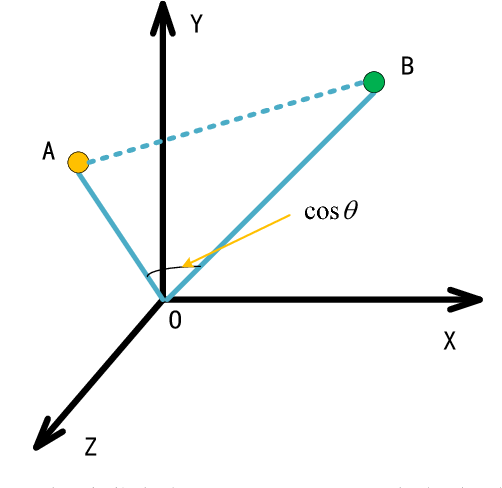
\includegraphics[scale=.3]{3Dspace.png}
	\label{fig:KNN}
\end{figure}

We applied two content-based recommendation systems using cosine similarity:
\begin{enumerate}
	\item
		\textbf{Movie Overviews and Taglines - uses ${movies\_metadata}$ file.}
		This system works on the overview and tagline attributes from the movies metadata file and considers those as description of the movie. This description is then used passed to TF-IDF encoding scheme to find the weights of the words in each of the description.
		\begin{figure}[h!]
			\centering
			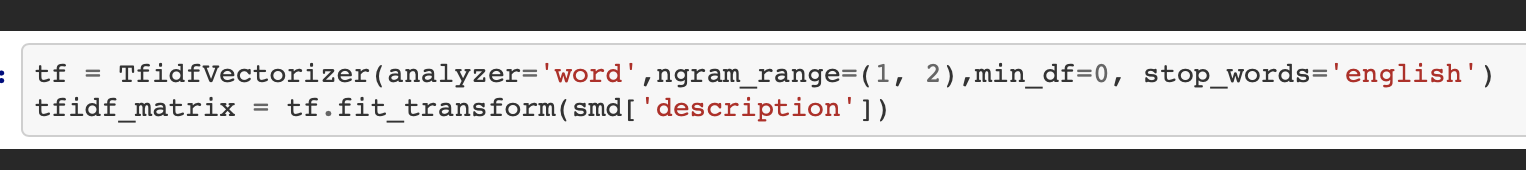
\includegraphics[scale=.3]{tfidf.png}
			\label{fig:Tf-IDF}
		\end{figure}
		These encoded movie vectors are then passed to the ${linear\_kernel}$ function to find the cosine similarities as this function works faster for large matrix. 
		\begin{figure}[h!]
			\centering
			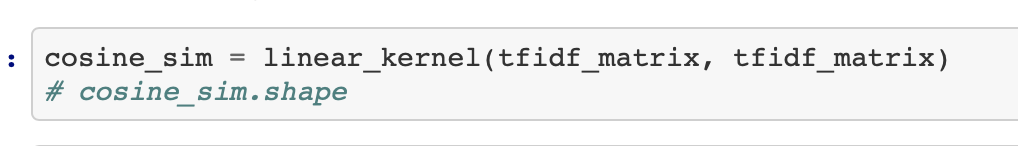
\includegraphics[scale=.5]{cosine_linear.png}
			\label{fig:Linear Kernel}
		\end{figure}
		The obtained cosine similarity matrix is later used to recommend the movie to the user using the following function: 
		\begin{figure}[h!]
			\centering
			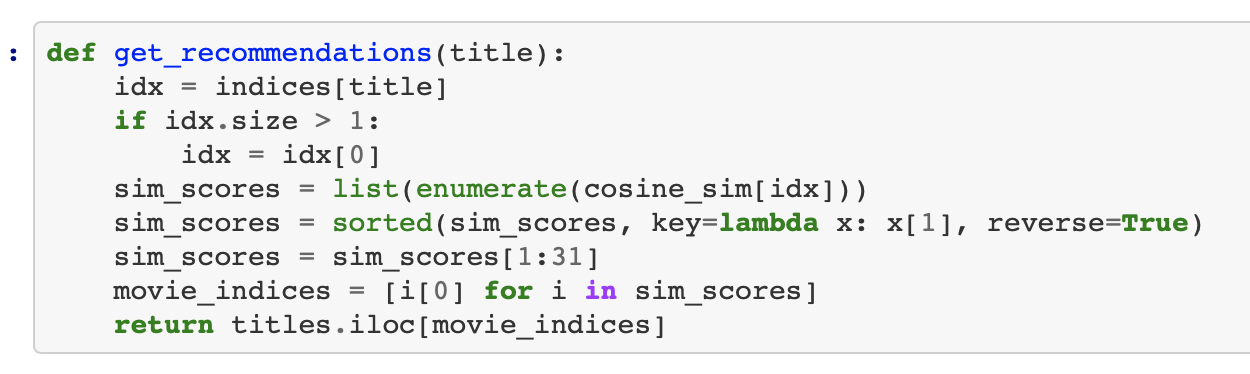
\includegraphics[scale=.4]{recommendation.png}
			\label{fig:Get_recommendation}
		\end{figure}

		\textbf{Output: (Using Movies)}
		\begin{figure}[H]
			\centering
			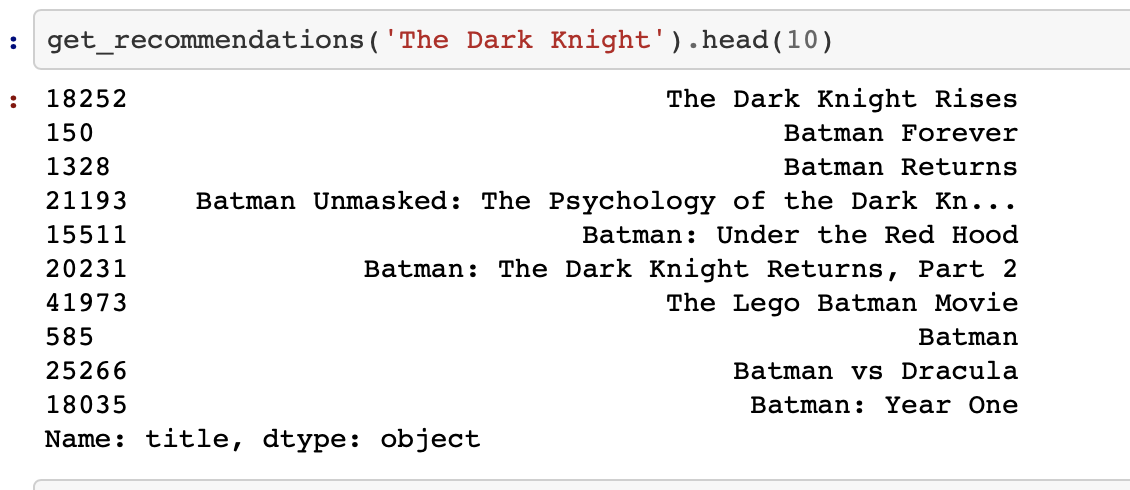
\includegraphics[scale=.3]{rec.png}
			\label{fig:Output 1}
		\end{figure}
	\item
		\textbf{Movie Cast, Crew, Keywords and Genre.}
		This uses the credits file and the keywords file.
		It uses cast, crew, keywords and genre of the movies and makes a sample metadata for each movies with this information.
		This sample metadata is then used passed to Count Vectorizer to create a count matrix.
		The count matrix is passed to the cosine\_similarity function to generate the cosine similarity matrix, which is further used in the same recommendation function which we used for the description-based recommender.
		\begin{figure}[h!]
			\centering
			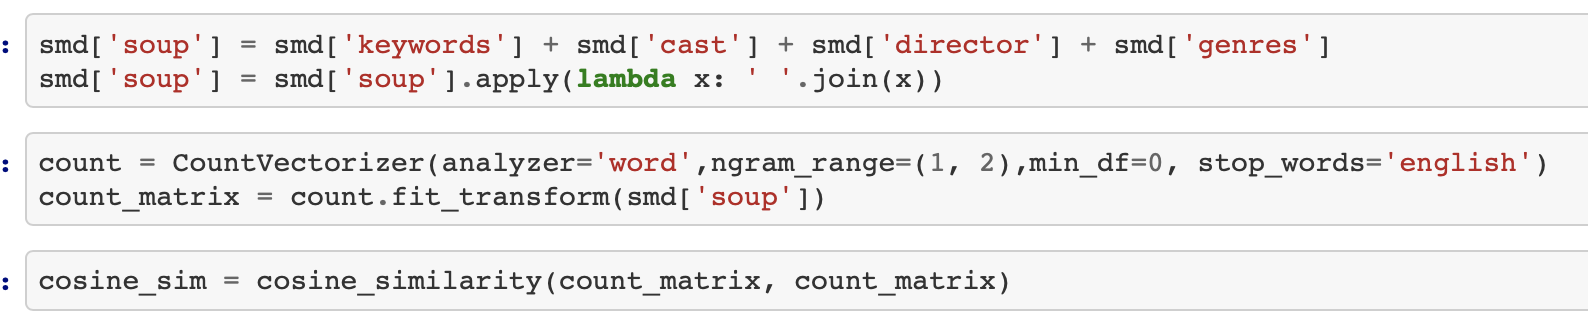
\includegraphics[scale=.3]{cosine_sim.png}
			\label{fig:Cosine Similarity}
		\end{figure}
		
		\textbf{Output: (Using Keywords)}
		\begin{figure}[H]
			\centering
			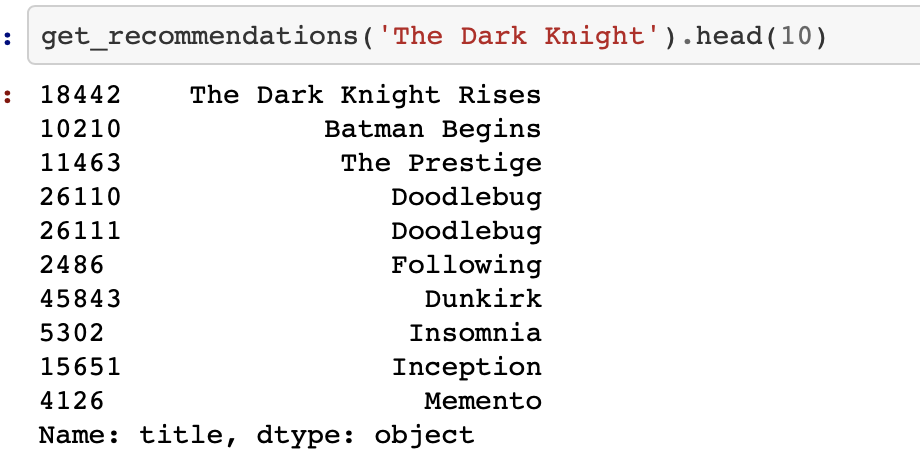
\includegraphics[scale=.3]{rec_keyword.png}
			\label{fig:Keyword Output}
		\end{figure}
		\textbf{Further Work:}
		Further, we have used the generated cosine similarity matrix (using keywords) in improved\_recommendation function, which sorts the most similar movies based on the weighted ratings of the movies.
		It uses vote\_count, vote\_averages, title and year from the movies\_metadata file and recommends the movies on the basis of the similar weighted ratings.
		\begin{figure}[H]
			\centering
			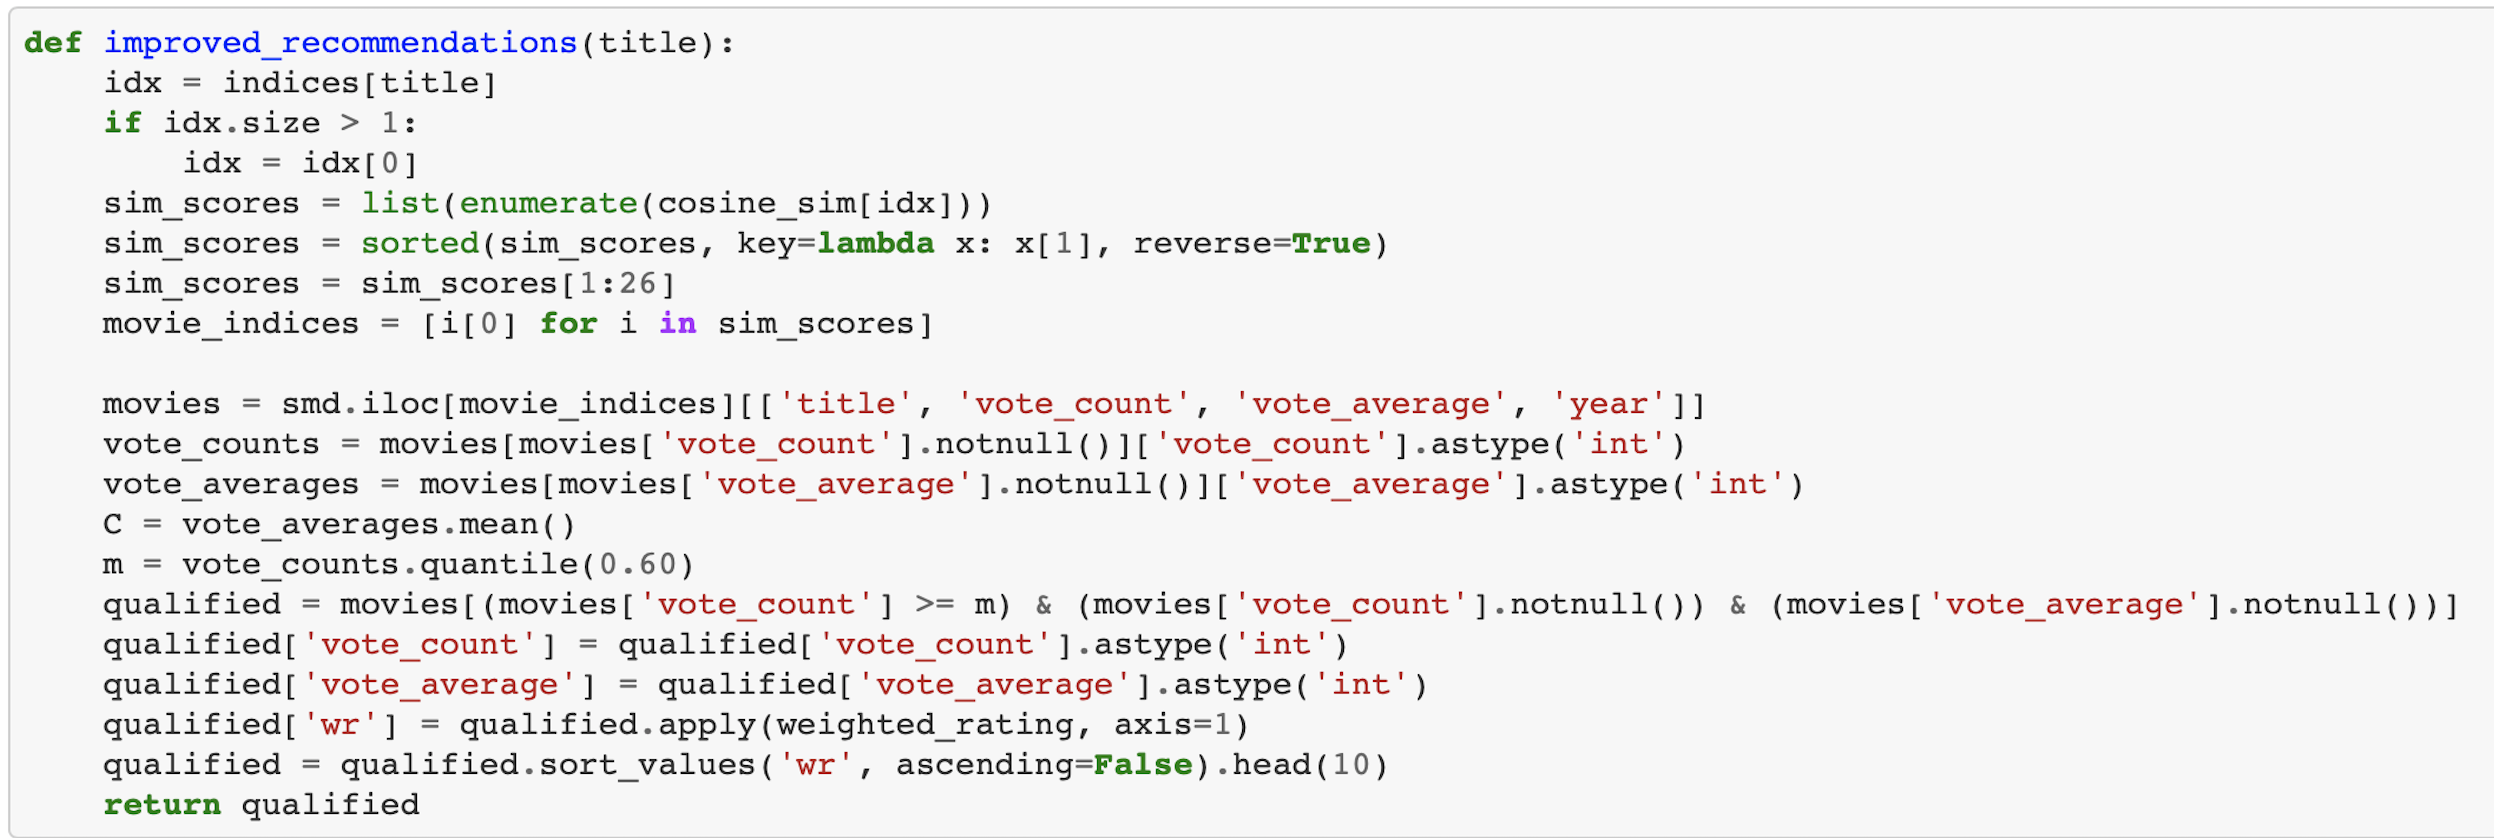
\includegraphics[scale=.2]{ratings.png}
			\label{fig:Rating Recommendation}
		\end{figure}

		\textbf{Output: (Using Keywords and Ratings)}
		\begin{figure}[H]
			\centering
			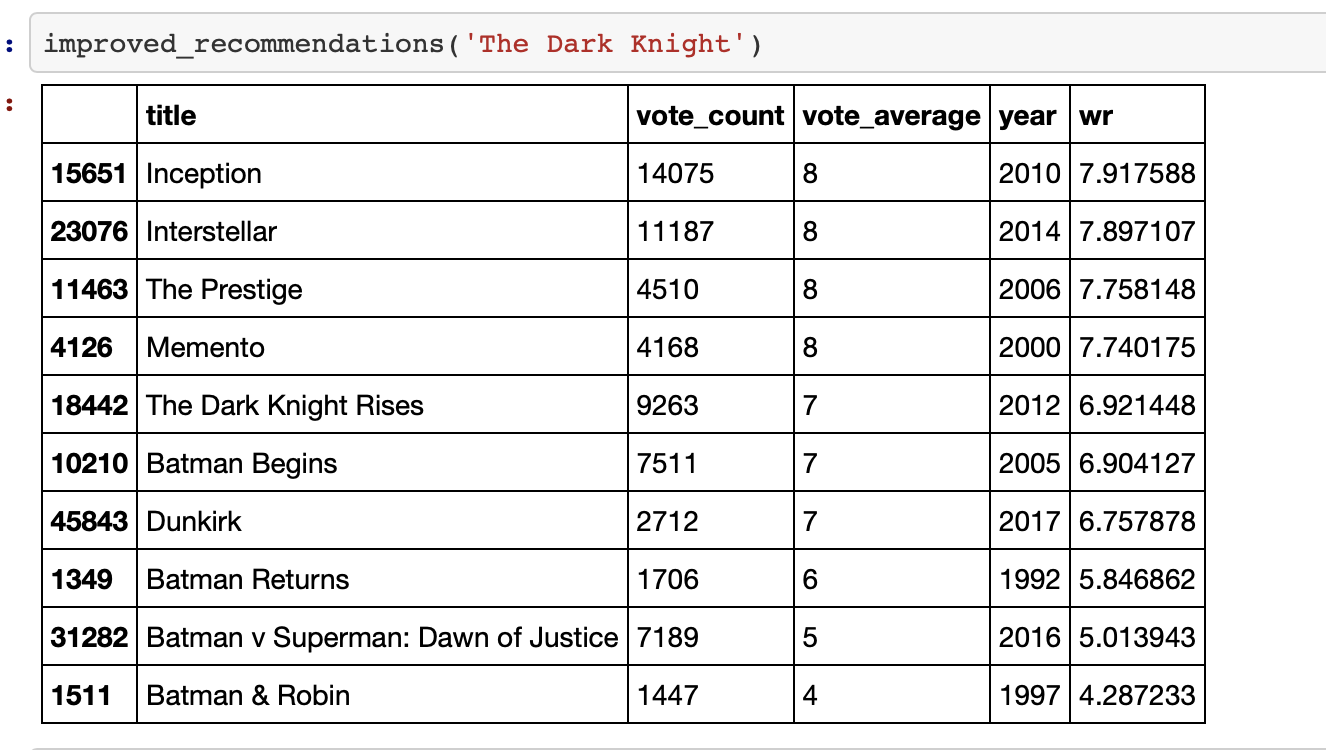
\includegraphics[scale=.3]{rec_rating.png}
			\label{fig:Rating Output}
		\end{figure}
\end{enumerate}

\subsection{\textbf{Item-Based Collaborative Filtering Method:}}
\begin{itemize}
	\item
		\textbf{KNN Algorithm:}
		In this recommendation system, K-Nearest Neighbors algorithm is used and the items will be clustered based on rating of item given by users and items were recommended based on similarity.\\
		KNN is a model that classifies data points based on the points that are most similar to it. KNN works as it uses the deeply rooted mathematical theories it. When implementing KNN, the first step is to transform data points into feature vectors, or their mathematical value. The algorithm then works by finding the distance between the mathematical values of these points. The most common way to find this distance is the Euclidean distance:
\begin{figure}[H]
\centering
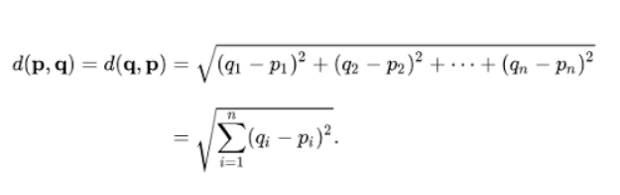
\includegraphics[scale=.6]{knn.png}
\label{fig:KNN}
\end{figure}
KNN runs this formula to compute the distance between each data point and the test data. It then finds the probability of these points being similar to the test data and classifies it based on which points share the highest probabilities. \\\\
  \item \textbf{SVD Approach:}
The factorization of a matrix into three matrices is known as singular vector decomposition. Here we consider a matrix A as a transformation that acts on a vector x by multiplication to produce a new vector Ax. The SVD of an ${m{\ast}n}$ matrix A with real values is a factorization of A as ${U \sum V^{T}}$, where U is an ${m{\ast}m}$ orthogonal matrix, V is a ${n{\ast}n}$ orthogonal matrix, and $\sum$ is a diagonal matrix with non-negative real entries on the diagonal.\\\\
\textbf{Key terms:} 
\begin{enumerate}
 \item span - basically gives us the entire range of possible values that you can get by multiplying each vector in a set of vectors by any real coefficient and then adding these values up (each of these combinations is called a linear combination).
 \item Orthogonal - means perpendicular but in multi-dimensional space. In the  movie-lens data we have key features such as ${User\_Id}$, ${Movie\_Id}$ and Ratings. Our task is to sort the movie recommendations based on these three traits.
\end{enumerate}
These features particularly create noise in the data. SVD here identifies a relevant sub-space of all the dimensions created by the noise in the data. The SVD finds an optimal line in multi-dimensional space that allows it to classify the data in the simplest way. Here, n = 3 total number of dimensions, the SVD algorithm will best fit in n-1 dimensions. Then in n-2, n-3. As the value of n goes down, SVD moves from weaker approximations to stronger approximations of the data.\\
The singular values go down with each dimension, which tells us that each dimension is adding less and less value. Our goal is to stop adding dimensions to our approximation when the singular values become relatively negligible.\\
In the implementation, we have used sk-learn library SVD method to, implement our movie recommendations based on the ${User\_Id}$, ${Movie\_Id}$ and Ratings. \\\\
\textbf{Error:}
\begin{figure}[H]
\centering
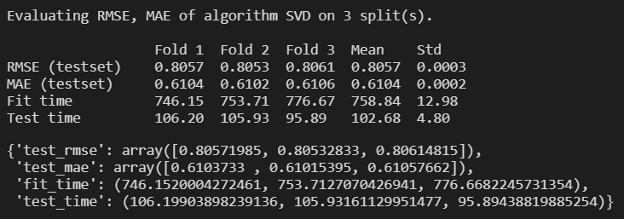
\includegraphics[scale=.5]{error.png}
\label{fig:error}
\end{figure}

\textbf{Prediction:} This will be clearer in the hybrid model.
\begin{figure}[H]
\centering
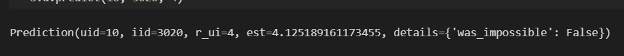
\includegraphics[scale=.5]{prediction.png}
\label{fig:Prediction}
\end{figure}
Now, building a universal hybrid model recommend movies based on a particular user. Here, we have computed a cosine similarity matrix for the movie metadata namely, keywords, cast, directors, crew etc. and we have created a recommendation function which takes ${user\_id}$ and movie name as input and recommends similar movies to the particular user. \\
Here is a snippet of the function: \\
\begin{figure}[H]
\centering
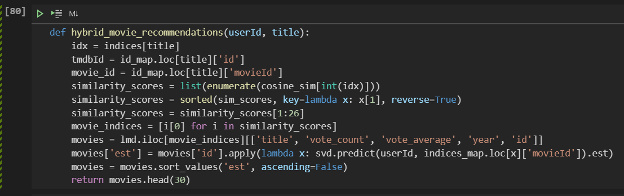
\includegraphics[scale=.5]{function.png}
\label{fig:Function}
\end{figure}
\textbf{Output:} Here is the output: (This recommendations are for ${user\_id}$ 3000 and movie The Godfather)
\begin{figure}[H]
\centering
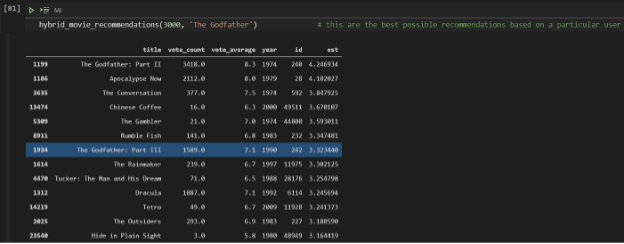
\includegraphics[scale=.5]{output.png}
\label{fig:Output}
\end{figure}
The hybrid model utilizes the entire dataset and gives its recommendations.
\end{itemize}

\section{Development}\label{sec:4. Development}
The website gives the user recommendations for movies based on a single movie. The image below is a screenshot of the website in use. Users can write the name of a movie, and the website will show different lists of recommendations. Each list is based on a slightly different source; one is for keywords and the other is for popularity.

\begin{figure}[H]
\centering
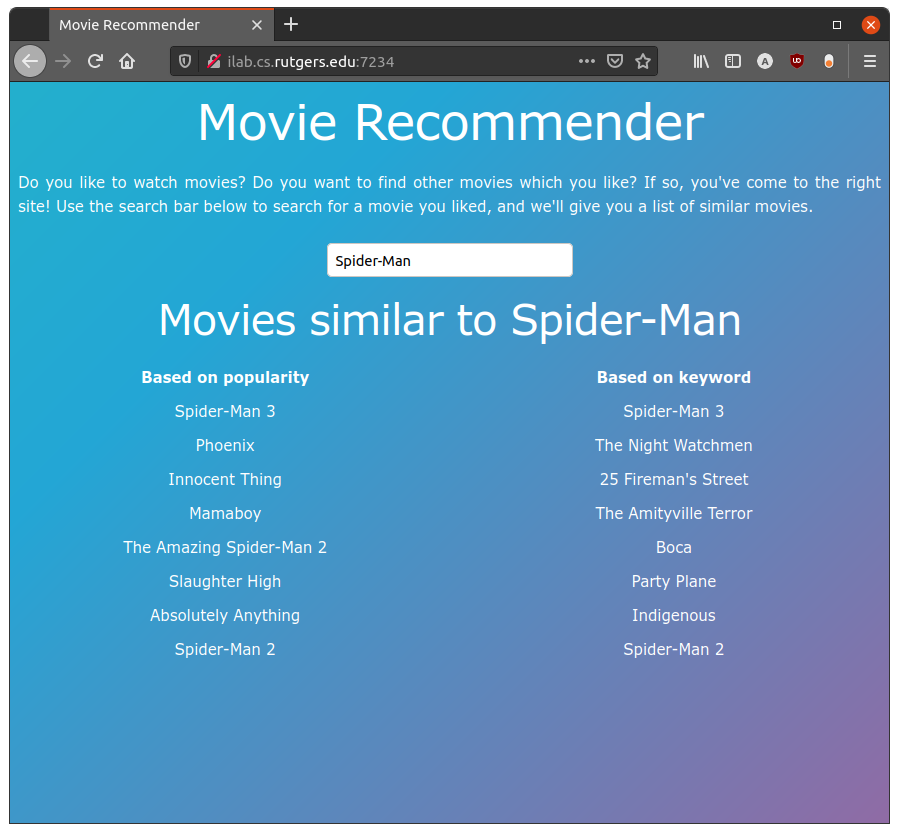
\includegraphics[scale=.25]{MovieRecommendation.png}
\label{fig:Movie Recommendation frontend}
\end{figure}

\subsection{\textbf{Frontend}}
The front-end for the website is built in HTML, CSS, and JavaScript. We chose not to use any frameworks like React.js or Vue.js because the website is so simple that we can write the code more cleanly with vanilla JS. In total, the front-end comprises only 96 lines of code.\\\\
When the user writes a movie in the search box, the front-end sends an AJAX request to the back-end. The back-end exposes an endpoint, /recommendation, which accepts arguments for the query movie and the technique to use (e.g. keywords or popularity). After the back-end returns the recommendations list, the front-end displays the recommendations in a list. This way, we do not need to reload the entire page, which feels much more comfortable for the users.\\\\
We also added a gradient animation as a background for the website. Gradient backgrounds are in fashion now, and they will probably stay popular for a few years.
\subsection{\textbf{Backend}}
The back-end is written using Python with Flask. We tried writing a server in Django instead of Flask, but we found that the Django server delivered the same capabilities as the Flask server while being much more complicated and harder to understand. Our final server is contained in a single file of 101 lines of code.\\\\
It exposes a static directory to serve the front-end and a single endpoint, /recommendation. The recommendation endpoint gives recommendations using a cosine similarity matrix. Our cosine similarity matrix is over 20 GB large, so we do not store the entire matrix in memory. Instead, when the user asks for recommendations for a movie, we only read the line of the matrix file corresponding to that movie. This way, we avoid the massive overhead of loading the entire matrix into memory. We also make the code scale better in memory; we use ${O(n)}$ memory where n is the number of movies whereas loading the entire matrix would use ${O(n^2)}$ memory.\\\\
One big challenge is reading the line from disk to memory. Although reading a line is much faster than reading the entire file, it still takes a few seconds. In the future, we want to use a different technique to read a single line from the file, or we would replace the file storage with a database.

\section{Conclusion}\label{sec:5. Conclusion}
In this project, we applied both content-based filtering and item-based collaborative filtering to build the recommendation system using the MovieLens Dataset. For the content-based filtering, we used cosine similarity method and found the similar movies on two different metrics; i.e, one based on similar movie description and other based on similar keywords, cast, crew, genre and ratings of the movie. For the item-based collaborative filtering approach, we used KNN algorithm and SVD, from which we got approximately ${80\%}$ accuracy. Further we have also made a hybrid recommendation system which uses cosine similarity matrix based on keywords and SVD to make recommendations. After comparing the results for each movie recommender, we considered cosine similarity approach gave us better results than other methods and so we have then used them for our webpage. For the further work, we plan to consider the working of other advanced recommendation approaches to improve our results.

\section{References}\label{sec:6. References}
\begin{enumerate}
  \item https://www.kaggle.com/gspmoreira/recommender-systems-in-python-101
  \item https://www.kaggle.com/vipulgandhi/pca-beginner-s-guide-to-dimensionality-reduction/comments
  \item https://towardsdatascience.com/recommender-system-application-development-part-1-of-4-cosine-similarity-f6dbcd768e83
  \item https://towardsdatascience.com/recommender-system-application-development-part-1-of-4-cosine-similarity-f6dbcd768e83
  \item https://www.youtube.com/watch?v=ueKXSupHz6Q
  \item https://www.kaggle.com/muhammadayman/recommendation-system-using-cosine-similarity?scriptVersionId=58384845
\end{enumerate}
\bibliographystyle{IEEEtran}
\end{document}


